\ifx\wholebook\relax \else

\documentclass[b5paper]{article}
\usepackage[nomarginpar
  %, margin=.5in
]{geometry}

\addtolength{\oddsidemargin}{-0.05in}
\addtolength{\evensidemargin}{-0.05in}
\addtolength{\textwidth}{0.1in}

\usepackage[en]{../../../prelude}

\setcounter{page}{1}

\begin{document}

\title{AVL tree}

\author{Xinyu LIU
\thanks{{\bfseries Xinyu LIU} \newline
  Email: liuxinyu95@gmail.com \newline}
  }

\maketitle
\fi

\markboth{AVL tree}{Elementary Algorithms}

\ifx\wholebook\relax
\chapter{AVL tree}
\numberwithin{Exercise}{chapter}
\fi

\section{Introduction}
\label{introduction} \index{AVL tree}

The idea of red-black tree is to limit the number nodes along a path within a range. AVL tree takes a direct approach: quantify the difference between branches. For a node $T$, define:

\be
  \delta(T) = |r| - |l|
\ee

Where $|T|$ is the height of tree $T$, $l$ and $r$ are the left and right sub-trees. Define $\delta(\nil) = 0$ for the empty tree. If $\delta(T) = 0$ for every node $T$, the tree is definitely balanced. For example, a complete binary tree has $n=2^h - 1$ nodes for height $h$. There are not any empty branches unless the leaves. The less absolute value of $\delta(T)$, the more balanced between the sub-trees. We call $\delta(T)$ the {\em balance factor} of a binary tree.

\section{Definition}
\index{AVL tree!definition}

\begin{figure}[htbp]
   \centering
   \includegraphics[scale=0.5]{img/avl-example.ps}
   \caption{an AVL tree}
   \label{fig:avl-example}
\end{figure}

A binary search tree is an AVL tree if all sub-trees satisfy:

\be
  |\delta(T)| \leq 1
\ee

There are three valid values for $\delta(T)$: $\pm 1$, and 0. Figure \ref{fig:avl-example} shows an AVL tree. This definition ensures the tree height $h = O(\lg n)$, where $n$ is the number of nodes in the tree. Let's prove it. For an AVL tree of height $h$, the number of nodes varies. There are at most $2^h - 1$ nodes for a complete binary tree case. We are interesting in how many nodes at least. Let the minimum number be $N(h)$. We have the following result:

\begin{itemize}
\item Empty tree $\nil$: $h = 0$, $N(0) = 0$;
\item Singleton tree: $h = 1$, $N(1) = 1$;
\end{itemize}

Figure \ref{fig:N-h-relation} shows an AVL tree $T$ of height $h$. It contains three parts, the key $k$, and two sub-trees $l$, $r$. We have the following equation:

\begin{figure}[htbp]
   \centering
   \includegraphics[scale=0.5]{img/Nh-lvr.ps}
   \caption{An AVL tree of height $h$. The height of one sub-tree is $h-1$, the other is no less than $h-2$.}
   \label{fig:N-h-relation}
\end{figure}

\be
  h = max(|l|, |r|) + 1
\ee

There must be a sub-tree of height $h - 1$. From the definition. we have $||l|-|r|| \leq 1$ holds. Hence the height of the other tree can not be lower than $h - 2$. The total number of the nodes in $T$ is the sum of both sub-trees plus 1 (for the root):

\be
  N(h) = N(h-1) + N(h-2) + 1
  \label{eq:Fibonacci-like}
\ee

This recursive equation is similar to Fibonacci numbers. Actually we can transform it to Fibonacci numbers through $N'(h) = N(h) + 1$. Equation (\ref{eq:Fibonacci-like}) then changes to:

\be
  N'(h) = N'(h-1) + N'(h-2)
\ee

\begin{lemma}
\label{lemma:N-phi}
Let $N(h)$ be the minimum number of nodes for an AVL tree of height $h$, and $N'(h) = N(h) + 1$, then
\be
  N'(h) \geq \phi^h
\ee

Where $\phi = \dfrac{\sqrt{5}+1}{2}$ is the golden ratio.
\end{lemma}

\begin{proof}
When $h = 0$ or 1, we have:
\begin{itemize}
\item $h = 0$: $N'(0) = 1 \geq \phi^0 = 1$
\item $h = 1$: $N'(1) = 2 \geq \phi^1 = 1.618...$
\end{itemize}

For the induction case, assume $N'(h) \geq \phi^h$.
\[
  \begin{array}{rll}
  N'(h+1) & = N'(h) + N'(h-1) & \{\text{Fibonacci}\} \\
          & \geq \phi^h + \phi^{h-1} & \\
          & = \phi^{h-1}(\phi + 1) & \{\phi + 1 = \phi^2 = \dfrac{\sqrt{5}+3}{2}\} \\
          & = \phi^{h+1}
 \end{array}
\]
\end{proof}

From Lemma \ref{lemma:N-phi}, we immediately obtain:

\be
  h \leq log_{\phi}(n+1) = log_{\phi}2 \cdot \lg (n+1) \approx 1.44 \lg (n+1)
  \label{eq:AVL-height}
\ee

We prove the height of AVL tree is proportion to $O(\lg n)$, indicating AVL tree is balanced.

When insert or delete, the balance factor may exceed the valid value range, we need fix to resume $|\delta|<1$. Traditionally, the fixing is through tree rotations. We give the simplified implementation based on pattern matching. The idea is similar to the functional red-black tree(Okasaki, \cite{okasaki}). Because of this `modify-fix' approach, AVL tree is also self-balanced binary search tree.

We can define AVL tree as algebraic data type with four cases\cite{hackage}: \texttt{E} for empty tree $\nil$, \texttt{N} for tree with $\delta = -1$, \texttt{P} for $\delta = 1$, and \texttt{Z} for $\delta = 0$. A direct way is to re-use the binary search tree definition. Although the balance factor $\delta$ can be computed recursively, we record it inside each node as $T = (l, k, r, \delta)$, and update it when mutate the tree\footnote{Alternatively, we can record the height instead of $\delta$\cite{py-avl}.}. Below example program adds $\delta$ as an \texttt{Int}:

\lstset{frame = single}
\begin{Haskell}
data AVLTree a = Empty
               | Br (AVLTree a) a (AVLTree a) Int
\end{Haskell}

For AVL tree, $lookup$, $max$, $min$ are as same as the binary search tree. We focus on $insert$ and $delete$ algorithms.

\section{Insert}
\index{AVL tree!insert}

When insert a new element, $|\delta(T)|$ may exceed 1. Traditional fixing uses tree rotation to maintain the balance factor in different cases. Alternatively, we can use pattern matching similar to red-black tree implementation\cite{okasaki} to develop a simplified solution.

After insert element $x$, for those sub-trees which are the ancestors of $x$, the height may increase at most by 1. We need recursively update the balance factor along the path of insertion. Define the insert result as a pair $(T', \Delta H)$, where $T'$ is the updated tree and $\Delta H$ is the increment of height. We modify the binary search tree $insert$ function for AVL tree as below:

\be
insert = \textit{fst} \circ ins
\ee

Where $\textit{fst}\ (a, b) = a$ returns the first element in a pair. $ins(T, k)$ does the actual work to insert element $k$ into tree $T$:

\be
\begin{array}{rcl}
ins\ \nil\ k & = & ((\nil, k, \nil, 0), 1) \\
ins\ (l, k', r, \delta)\ k & = & \begin{cases}
  k < k': tree\ (ins\ l\ k)\ k'\ (r, 0)\ \delta \\
  k > k': tree\ (l, 0)\ k'\ (ins\ r, k)\ \delta \\
\end{cases}
\end{array}
\label{eq:ins}
\ee

If the tree is empty $\nil$, the result is a leaf of $k$ with balance factor 0. The height increases to 1. Otherwise let $T = (l, k', r, \delta)$. We compare the new element $k$ with $k'$. If $k < k'$, we recursively insert $k$ it to the left sub-tree $l$, otherwise insert to the right. As the recursive insert result is a pair of $(l', \Delta l)$ or $(r', \Delta r)$, we need adjust the balance factor and update tree height through function $tree$, it takes 4 parameters: $(l', \Delta l)$, $k'$, $(r', \Delta r)$, and $\delta$. The result is $(T', \Delta H)$, where $T'$ is the tree after adjustment, and $\Delta H$ is the increment of height, defined as:

\be
  \Delta H = |T'| - |T|
\ee

We can further break it down into 4 cases:

\be
\begin{array}{rcl}
  \Delta H & = & |T'| - |T| \\
           & = & 1 + max(|r'|, |l'|) - (1 + max(|r|, |l|)) \\
           & = & max(|r'|, |l'|) - max(|r|, |l|) \\
           & = & \begin{cases}
\delta \geq 0, \delta' \geq 0: & \Delta r \\
\delta \leq 0, \delta' \geq 0: & \delta + \Delta r \\
\delta \geq 0, \delta' \leq 0: & \Delta l - \delta \\
otherwise: & \Delta l
\end{cases}
\end{array}
\ee

Where $\delta' = \delta(T') = |r'| - |l'|$, is the updated balance factor. Appendix B provides the proof for it. We need determine $\delta'$ before balance adjustment.

\be
\begin{array}{rcl}
\delta' & = & |r'| - |l'| \\
        & = & |r| + \Delta r - (|l| + \Delta l) \\
        & = & |r| - |l| + \Delta r - \Delta l \\
        & = & \delta + \Delta r - \Delta l \\
\end{array}
\ee

With the changes in height and balance factor, we can define the $tree$ function in (\ref{eq:ins}):

\be
tree\ (l', \Delta l)\ k\ (r', \Delta r)\ \delta =
  balance\ (l', k, r', \delta')\ \Delta H
\ee

Below example programs implements what we deduced so far:

\begin{Haskell}
insert t x = fst $ ins t where
    ins Empty = (Br Empty x Empty 0, 1)
    ins (Br l k r d)
        | x < k = tree (ins l) k (r,  0) d
        | x > k = tree (l,  0) k (ins r) d

tree (l, dl) k (r, dr) d = balance (Br l k r d') deltaH where
    d' = d + dr - dl
    deltaH | d >=0 && d' >=0 = dr
           | d <=0 && d' >=0 = d+dr
           | d >=0 && d' <=0 = dl - d
           | otherwise = dl
\end{Haskell}

\subsection{Balance}
\index{AVL tree!balance}
There are 4 cases need fix as shown in figure \ref{fig:avl-insert-fix}. The balance factor is $\pm 2$, exceeds the range of $[-1, 1]$. We adjust them to a uniformed structure in the center, with the $\delta(y) = 0$.

\begin{figure}[htbp]
  \centering
  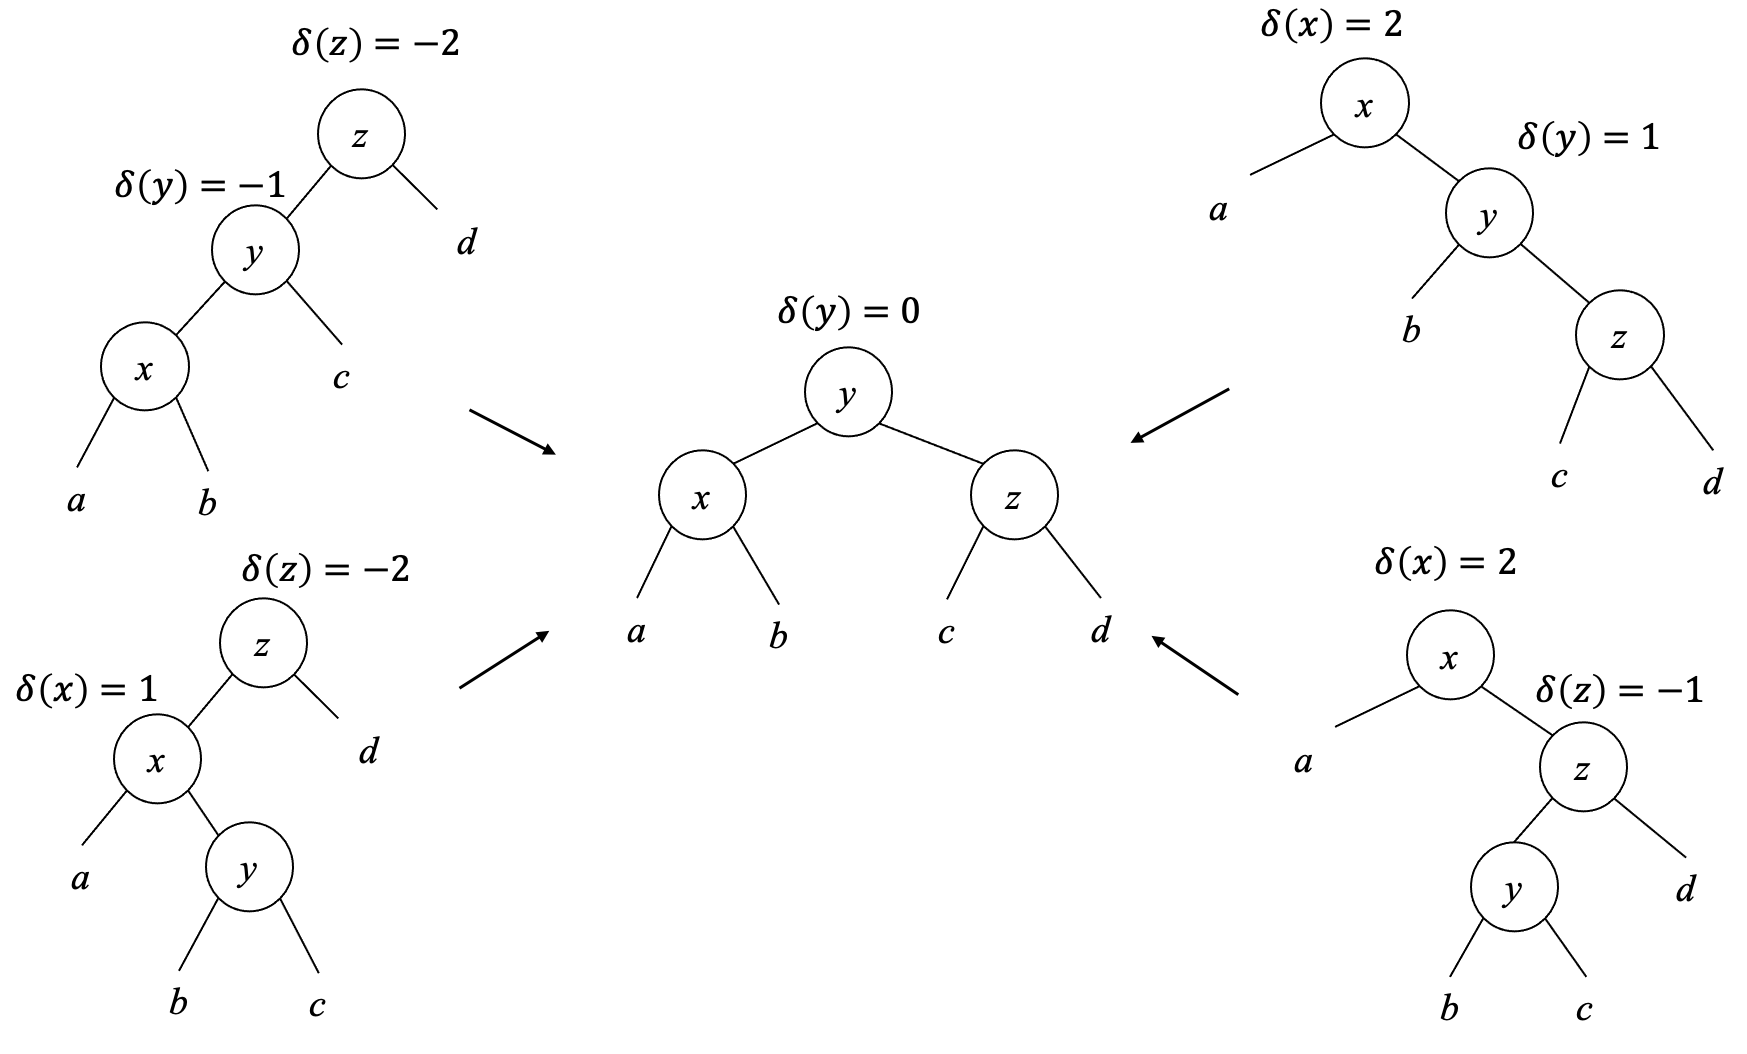
\includegraphics[scale=0.4]{img/avl-insert-fix.png}
  \caption{Fix 4 cases to the same structure}
  \label{fig:avl-insert-fix}
\end{figure}

We call the 4 cases: left-left, right-right, right-left, and left-right. Denote the balance factors before fixing as $\delta(x), \delta(y)$, and $\delta(z)$; after fixing, they change to $\delta'(x), \delta'(y) = 0$, and $\delta'(z)$ respectively. The values of $\delta'(x)$ and $\delta'(z)$ can be given as below. Appendix B gives the proof.

Left-left:

\be
  \begin{array}{l}
  \delta'(x) = \delta(x) \\
  \delta'(y) = 0 \\
  \delta'(z) = 0
  \end{array}
\ee

Right-right:

\be
  \begin{array}{l}
  \delta'(x) = 0 \\
  \delta'(y) = 0 \\
  \delta'(z) = \delta(z)
  \end{array}
  \label{eq:rr-result}
\ee

Right-left and Left-right:

\be
  \begin{array}{l}
  \delta'(x) = \begin{cases}
    \delta(y) = 1: & -1 \\
    otherwise: & 0 \\
    \end{cases} \\
  \delta'(y) = 0 \\
  \delta'(z) = \begin{cases}
    \delta(y) = -1: & 1 \\
    otherwise: & 0 \\
    \end{cases} \\
  \end{array}
  \label{eq:rl-result}
\ee

Based on this, we can implement the pattern matching fix as below:

\be
\resizebox{\textwidth}{!}{\ensuremath{
\begin{array}{rcl}
balance\ (((a, x, b, \delta(x)), y, c, -1), z, d, -2)\ \Delta H & = & ((a, x, b, \delta(x)), y, (c, z, d, 0), 0, \Delta H -1) \\
balance\ (a, x, (b, y, (c, z, d, \delta(z)), 1), 2)\ \Delta H & = & ((a, x, b, 0), y, (c, z, d, \delta(z)), 0, \Delta H -1) \\
balance\ ((a, x, (b, y, c, \delta(y)), 1), z, d, -2)\ \Delta H & = & ((a, x, b, \delta'(x)), y, (c, z, d, \delta'(z)), 0, \Delta H - 1) \\
balance\ (a, x, ((b, y, c, \delta(y)), z, d, -1), 2)\ \Delta H & = & ((a, x, b, \delta'(x)), y, (c, z, d, \delta'(z)), 0, \Delta H - 1) \\
balance\ T\ \Delta H & = & (T, \Delta H) \\
\end{array}
}}
\ee

Where $\delta'(x)$ and $delta'(z)$ are defined in (\ref{eq:rl-result}). If none of the pattern matches, the last row keeps the tree unchanged. Below is the example program implements $balance$:

\begin{Haskell}
balance (Br (Br (Br a x b dx) y c (-1)) z d (-2)) dH =
            (Br (Br a x b dx) y (Br c z d 0) 0, dH-1)
balance (Br a x (Br b y (Br c z d dz)    1)    2) dH =
            (Br (Br a x b 0) y (Br c z d dz) 0, dH-1)
balance (Br (Br a x (Br b y c dy)    1) z d (-2)) dH =
            (Br (Br a x b dx') y (Br c z d dz') 0, dH-1) where
    dx' = if dy ==  1 then -1 else 0
    dz' = if dy == -1 then  1 else 0
balance (Br a x (Br (Br b y c dy) z d (-1))    2) dH =
            (Br (Br a x b dx') y (Br c z d dz') 0, dH-1) where
    dx' = if dy ==  1 then -1 else 0
    dz' = if dy == -1 then  1 else 0
balance t d = (t, d)
\end{Haskell}

The insertion algorithm takes time proportion to the height of the
tree. As AVL is balanced according to (\ref{eq:AVL-height}), its performance
is $O(\lg n)$ where $n$ is the number of elements stored in the AVL
tree.

\subsubsection{Verification}
\index{AVL tree!verification}
When verify if a tree is AVL tree, we need verify two things,
first, it's a binary search tree; second, it satisfies AVL tree property.

In order to test if a binary tree satisfies AVL tree property, we can
examine the height difference between the two sub trees recursively
till the leaves.

\be
  avl?(T) = \left \{
  \begin{array}
  {r@{\quad:\quad}l}
  True & T = \phi \\
  avl?(T_l) \land avl?(T_r) \land ||T_r|-|T_l|| \leq 1 & otherwise
  \end{array}
  \right .
\ee

Where the height can also be calculated recursively.

\be
  |T| = \left \{
  \begin{array}
  {r@{\quad:\quad}l}
  0 & T = \phi \\
  1 + max(|T_r|, |T_l|) & otherwise
  \end{array}
  \right .
\ee

The corresponding Haskell example program is given as the following.

\begin{lstlisting}
isAVL :: (AVLTree a) -> Bool
isAVL Empty = True
isAVL (Br l _ r d) = and [isAVL l, isAVL r, abs (height r - height l) <= 1]

height :: (AVLTree a) -> Int
height Empty = 0
height (Br l _ r _) = 1 + max (height l) (height r)
\end{lstlisting}

\begin{Exercise}
Write a program to verify if a tree is the AVL tree.
Please consider both functional and imperative approaches.
\end{Exercise}



% ================================================================
%                 Deletion
% ================================================================

\section{Deletion}
\index{AVL tree!deletion}

As we mentioned before, deletion will not be a major problem in
purely functional settings. As the tree is read only, the use case
is typically performing looking up after build.

For purely functional deletion, it actually re-builds the tree
as we show in the chatper of red-black tree. We put the AVL
tree deletion algorithm in Appendix C.

\section{Imperative AVL tree algorithm $\star$}
\index{AVL tree!imperative insertion}

This section shows the traditional insert-and-rotate
approach to realize AVL tree insertion algorithm.

Similar to the red-black tree algorithm, the strategy
is to first do the binary search tree insertion,
then fix the balance by rotation and return the final result.

\begin{algorithmic}[1]
\Function{Insert}{$T, k$}
  \State $root \gets T$
  \State $x \gets$ \Call{Create-Leaf}{$k$}
  \State \Call{$\delta$}{$x$} $\gets 0$
  \State $parent \gets$ NIL
  \While{$T \neq$ NIL}
    \State $parent \gets T$
    \If{$k <$ \Call{Key}{$T$}}
      \State $T \gets $ \Call{Left}{$T$}
    \Else
      \State $T \gets $ \Call{Right}{$T$}
    \EndIf
  \EndWhile
  \State \Call{Parent}{$x$} $\gets parent$
  \If{$parent =$ NIL} \Comment{tree $T$ is empty}
    \State \Return $x$
  \ElsIf{$k <$ \Call{Key}{$parent$}}
    \State \Call{Left}{$parent$} $\gets x$
  \Else
    \State \Call{Right}{$parent$} $\gets x$
  \EndIf
  \State \Return \Call{AVL-Insert-Fix}{$root, x$}
\EndFunction
\end{algorithmic}

Note that after insertion, the balance factor $\delta$ may change because
the height of the tree can grow. Inserting on right side can
increase $\delta$ by 1, while insert on left side can decrease it. By
the end of this algorithm, we need perform bottom-up fixing from node $x$
towards root.

We can translate the pseudo code to Python example program\footnote{C and C++ source code are available along with this book}.
\lstset{language=Python}
\begin{lstlisting}
def avl_insert(t, key):
    root = t
    x = Node(key)
    parent = None
    while(t):
        parent = t
        if(key < t.key):
            t = t.left
        else:
            t = t.right
    if parent is None: #tree is empty
        root = x
    elif key < parent.key:
        parent.set_left(x)
    else:
        parent.set_right(x)
    return avl_insert_fix(root, x)
\end{lstlisting}

This is a top-down algorithm. It searches the tree from root down to the proper
position and inserts the new key as a leaf. By the end of this algorithm, it calls the fixing function with the root and the new inserted node.

Note that we reuse the same methods of \texttt{set\_left()} and \texttt{set\_right()} as
we defined in chapter of red-black tree.

In order to resume the AVL tree property, we first check if the new node is inserted on left or right. If it is on left, the balance factor $\delta$ decreases, otherwise it increases. If we denote the new value as $\delta'$, there are 3 cases between $\delta$ and $\delta'$.

\begin{itemize}
\item If $|\delta| = 1$ and $|\delta'| = 0$, it means the new node makes the tree perfectly balanced, the height of the parent node doesn't change, the algorithm can be terminated.

\item If $|\delta| = 0$ and $|\delta'| = 1$, it means either the left or the right sub tree increases its height. We need go on checking the upper level of the tree.

\item If $|\delta| = 1$ and $|\delta'| = 2$, it means the AVL tree property is violated due to the new insertion. We need perform rotation to fix it.
\end{itemize}

\begin{algorithmic}[1]
\Function{AVL-Insert-Fix}{$T, x$}
  \While{\Call{Parent}{$x$} $\neq$ NIL}
    \State $\delta \gets $ \textproc{$\delta$}(\Call{Parent}{$x$})
    \If{$x = $ \textproc{Left}(\Call{Parent}{$x$})}
      \State $\delta' \gets \delta - 1$
    \Else
      \State $\delta' \gets \delta + 1$
    \EndIf
    \State \textproc{$\delta$}(\Call{Parent}{$x$}) $\gets \delta'$
    \State $P \gets $ \Call{Parent}{$x$}
    \State $L \gets $ \Call{Left}{$x$}
    \State $R \gets $ \Call{Right}{$x$}
    \If{$|\delta| = 1$ and $|\delta'| = 0$} \Comment{Height doesn't change, terminates.}
      \State \Return $T$
    \ElsIf{$|\delta| = 0$ and $|\delta'| = 1$} \Comment{Go on bottom-up updating.}
      \State $x \gets P$
    \ElsIf{$|\delta| = 1$ and $|\delta'| = 2$}
      \If{$\delta'=2$}
        \If{$\delta(R) = 1$} \Comment{Right-right case}
          \State $\delta(P) \gets 0$ \Comment{By (\ref{eq:rr-result})}
          \State $\delta(R) \gets 0$
          \State $T \gets $ \Call{Left-Rotate}{$T, P$}
        \EndIf
        \If{$\delta(R) = -1$} \Comment{Right-left case}
          \State $\delta_y \gets $ \textproc{$\delta$}(\Call{Left}{$R$}) \Comment{By (\ref{eq:rl-result})}
          \If{$\delta_y = 1$}
            \State $\delta(P) \gets -1$
          \Else
            \State $\delta(P) \gets 0$
          \EndIf
          \State \textproc{$\delta$}(\Call{Left}{$R$}) $\gets 0$
          \If{$\delta_y = -1$}
            \State $\delta(R) \gets 1$
          \Else
            \State $\delta(R) \gets 0$
          \EndIf
          \State $T \gets $ \Call{Right-Rotate}{$T, R$}
          \State $T \gets $ \Call{Left-Rotate}{$T, P$}
        \EndIf
      \EndIf
      \If{$\delta' = -2$}
        \If{$\delta(L) = -1$} \Comment{Left-left case}
          \State $\delta(P) \gets 0$
          \State $\delta(L) \gets 0$
          \State \Call{Right-Rotate}{$T, P$}
        \Else \Comment{Left-Right case}
          \State $\delta_y \gets $ \textproc{$\delta$}(\Call{Right}{$L$})
          \If{$\delta_y = 1$}
            \State $\delta(L) \gets -1$
          \Else
            \State $\delta(L) \gets 0$
          \EndIf
          \State \textproc{$\delta$}(\Call{Right}{$L$}) $\gets 0$
          \If{$\delta_y = -1$}
            \State $\delta(P) \gets 1$
          \Else
            \State $\delta(P) \gets 0$
          \EndIf
          \State \Call{Left-Rotate}{$T, L$}
          \State \Call{Right-Rotate}{$T, P$}
        \EndIf
      \EndIf
      \State break
    \EndIf
  \EndWhile
  \State \Return $T$
\EndFunction
\end{algorithmic}

As rotation operation doesn't update the balance factor $\delta$,
we need update it for impacted nodes. Among the four cases, the right-right case and the left-left case need only one rotation, while the right-left case and the left-right case need two rotations.

The relative example python program is as the following.

\begin{lstlisting}
def avl_insert_fix(t, x):
    while x.parent is not None:
        d2 = d1 = x.parent.delta
        if x == x.parent.left:
            d2 = d2 - 1
        else:
            d2 = d2 + 1
        x.parent.delta = d2
        (p, l, r) = (x.parent, x.parent.left, x.parent.right)
        if abs(d1) == 1 and abs(d2) == 0:
            return t
        elif abs(d1) == 0 and abs(d2) == 1:
            x = x.parent
        elif abs(d1)==1 and abs(d2) == 2:
            if d2 == 2:
                if r.delta == 1:  # Right-right case
                    p.delta = 0
                    r.delta = 0
                    t = left_rotate(t, p)
                if r.delta == -1: # Right-Left case
                    dy = r.left.delta
                    if dy == 1:
                        p.delta = -1
                    else:
                        p.delta = 0
                    r.left.delta = 0
                    if dy == -1:
                        r.delta = 1
                    else:
                        r.delta = 0
                    t = right_rotate(t, r)
                    t = left_rotate(t, p)
            if d2 == -2:
                if l.delta == -1: # Left-left case
                    p.delta = 0
                    l.delta = 0
                    t = right_rotate(t, p)
                if l.delta == 1: # Left-right case
                    dy = l.right.delta
                    if dy == 1:
                        l.delta = -1
                    else:
                        l.delta = 0
                    l.right.delta = 0
                    if dy == -1:
                        p.delta = 1
                    else:
                        p.delta = 0
                    t = left_rotate(t, l)
                    t = right_rotate(t, p)
            break
    return t
\end{lstlisting}

We put the AVL tree deletion algorithm in appendix C for reference.

\section{Chapter note}
AVL tree was invented in 1962 by Adelson-Velskii and Landis\cite{wiki-avl},
\cite{TFATP}. The name AVL tree comes from the two inventor's name. It's earlier than red-black tree.

It's very common to compare AVL tree and red-black tree, both are self-balancing binary search trees, and for all the major operations, they both consume $O(\lg n)$ time. From the result of (\ref{eq:AVL-height}), AVL tree is more rigidly balanced hence they are faster than red-black tree in looking up intensive applications \cite{wiki-avl}. However, red-black trees could perform better in frequently insertion and removal cases.

Many popular self-balancing binary search tree libraries are implemented on top of red-black tree such as STL etc. However, AVL tree provides an intuitive and effective solution to the balance problem as well.

After this chapter, we'll extend the tree data structure from storing data in node to storing information on edges. It leads to Radix trees. If we extend the number of children from two to more, we can get B-tree. These data structures will be introduced in the next chapters.

\section{Appendix: Example programs}

Definition of AVL tree node.

\begin{lstlisting}[language = Bourbaki]
data Node<T> {
    int delta
    T key
    Node<T> left
    Node<T> right
    Node<T> parent
}
\end{lstlisting}


\begin{thebibliography}{99}

\bibitem{hackage}
Data.Tree.AVL \url{http://hackage.haskell.org/packages/archive/AvlTree/4.2/doc/html/Data-Tree-AVL.html}

\bibitem{okasaki}
Chris Okasaki. ``FUNCTIONAL PEARLS Red-Black Trees in a Functional Setting''. J. Functional Programming. 1998

\bibitem{wiki-avl}
Wikipedia. ``AVL tree''. \url{http://en.wikipedia.org/wiki/AVL_tree}

\bibitem{TFATP}
Guy Cousinear, Michel Mauny. ``The Functional Approach to Programming''. Cambridge University Press; English Ed edition (October 29, 1998). ISBN-13: 978-0521576819

\bibitem{py-avl}
Pavel Grafov. ``Implementation of an AVL tree in Python''. \url{http://github.com/pgrafov/python-avl-tree}
\end{thebibliography}

\ifx\wholebook\relax\else
\end{document}
\fi

% LocalWords:  AVL Okasaki STL
